%------------------------------------------------
%	PACKAGES AND THEMES
%------------------------------------------------

% this is a 4:3 layout.
\documentclass{beamer}
% for 16:9 use this command:
% \documentclass[aspectratio=169]{beamer}

\mode<presentation> {
\usetheme{metropolis}
\setbeamertemplate{caption}[numbered]
\setbeamertemplate{navigation symbols}{} % hide navigation symbols
}

\usepackage{graphicx} % images
\usepackage{algorithm2e}
\usepackage{mathtools}
\DeclarePairedDelimiter{\ceil}{\lceil}{\rceil}
\usepackage{algpseudocode}
\usepackage{booktabs} % allows the use of \toprule, \midrule and \bottomrule in tables
\usepackage[ngerman]{babel}
\usepackage[utf8]{inputenc}
\usepackage[T1]{fontenc}
\usepackage{mathtools}
\usepackage{xcolor}
\usepackage{listings} % code
\usepackage{pgf,tikz} % drawing
\usepackage{pifont} % new symbols
\usepackage{hyperref} % pretty links
% \usepackage{algorithmicx}
% \usepackage{algpseudocode}
% \usepackage[linesnumbered,ruled]{algorithm2e}

\usepackage{lmodern}
\usepackage{subcaption}
\usepackage{textcomp}
% \usepackage{array}
% \usepackage{longtable}
% \usepackage{verbatim}
%\usepackage{tabularx}
\captionsetup[figure]{font=footnotesize}

\usepackage{amsmath}
\usepackage{amssymb}
\usepackage{amsthm}
% \usepackage{comment}
% \usepackage{enumitem}
% \usepackage[binary-units=true]{siunitx}
% \usepackage{thmtools}
\usepackage{csquotes}
\usepackage{tikz}
\usepackage{float}
\usetikzlibrary{automata,positioning}

% color settings for links
\hypersetup{
    colorlinks=true,
    urlcolor=blue,
    linkcolor=black,
    citecolor=green!50!black
}

\definecolor{mygreen}{RGB}{1,135,1}

\newcommand{\cmark}{\ding{51}}  % checkmark
\newcommand{\xmark}{\ding{55}}  % xmark
\newcommand\scalemath[2]{\scalebox{#1}{\mbox{\ensuremath{\displaystyle #2}}}}

% \useoutertheme{miniframes} % navigation design
\useinnertheme{circles} % use non shiny circles (itemize, etc.)

% Main slide colors
% dunkel, hell, mittel
% \definecolor{pale}{RGB}{232, 236, 237}
% \definecolor{prim}{RGB}{53, 109, 120}
% \definecolor{sec}{RGB}{104, 170, 183}
% \definecolor{tert}{RGB}{109, 155, 168}
% \definecolor{quat}{RGB}{9, 59, 68}

\definecolor{pale}{RGB}{232, 236, 237}
% \definecolor{prim}{RGB}{153, 194, 173}
% good: \definecolor{prim}{RGB}{27, 33, 42}
\definecolor{prim}{RGB}{32, 43, 50}
\definecolor{sec}{RGB}{217, 232, 224}
\definecolor{tert}{RGB}{0, 82, 41}
% save
\definecolor{quat}{RGB}{0, 82, 41}

\setbeamercolor{palette primary}{bg=prim,fg=pale}
\setbeamercolor{palette secondary}{bg=sec,fg=pale}
\setbeamercolor{palette tertiary}{bg=tert,fg=pale}
\setbeamercolor{palette quaternary}{bg=quat,fg=pale}
\setbeamercolor{structure}{fg=prim} % itemize, enumerate, etc
\setbeamercolor{section in toc}{fg=prim} % TOC sections

% Block colors
\definecolor{example_color}{RGB}{93, 137, 98}
\definecolor{alert_color}{RGB}{175, 79, 72}

\setbeamercolor{normal text}{fg=prim!20!black,bg=pale!25!white}
\setbeamercolor{alerted text}{fg=alert_color!25!black}
\setbeamercolor{example text}{fg=example_color!25!black}

\setbeamercolor{block title example}{fg=white,bg=example_color}
\setbeamercolor{block body example}{fg=black,bg=example_color!10!white}
\setbeamercolor{block title alerted}{fg=white,bg=alert_color}
\setbeamercolor{block body alerted}{fg=black,bg=alert_color!10!white}

% Override palette coloring
\setbeamercolor{subsection in head/foot}{bg=quat,fg=pale}

\setbeamertemplate{frametitle}{%
    \nointerlineskip%

    \begin{beamercolorbox}[wd=\paperwidth,ht=2.5ex,dp=1ex]{frametitle}
        \hspace*{1ex}\insertframetitle%
        \ifx\insertframesubtitle@empty\else%
        {~\tiny\textcolor{quat!35!black}{\insertframesubtitle}}%
        \fi%
    \end{beamercolorbox}%
}

% math-command for bigger norm
\newcommand\norm[1]{\left\lVert#1\right\rVert}

% use this to include other files
% in this case style definitions for code
% alternative: \include{dateiname}
\lstdefinestyle{latex}{
    language=[LaTeX]TeX,
    inputencoding=utf8,
    basicstyle=\ttfamily,
    keywordstyle=\color{blue!60!black}, % use 60 percent blue and 40 black
    commentstyle=\color{cyan!60!black},
    tabsize=2,
    emph={document,itemize,enumerate,center,tabular,table,
    figure,wrapfigure,minipage,columns,align,bmatrix,
    lstlisting,beamer,frame,tikzpicture},
    emphstyle=\color{magenta!60!black},
    morekeywords={lstset,includegraphics,theenumi,labelitemi,column,color,url,href}
}

\lstdefinestyle{inline_latex}{
    language=[LaTeX]TeX,
    inputencoding=utf8,
    basicstyle=\ttfamily,
    resetmargins= true,
    belowcaptionskip=0pt,
    aboveskip=0pt,
    belowskip=0pt,
    keywordstyle=\color{blue!60!black},
    commentstyle=\color{cyan!60!black},
    emph={document,itemize,enumerate,center,tabular,table,
    figure,wrapfigure,minipage,columns,align,bmatrix,
    lstlisting,beamer,frame,tikzpicture,Parameter},
    emphstyle=\color{magenta!60!black},
    morekeywords={lstset,includegraphics,theenumi,labelitemi,column,color,url,href,Befehlsname}
}

\lstdefinestyle{cpp}{
    language=C++,
    basicstyle=\ttfamily,
    keywordstyle=\color{blue!90!black},
    stringstyle=\color{magenta!60!black},
    commentstyle=\color{green!35!black},
    morecomment=[l][\color{gray!60!black}]{\#},
    tabsize=2
}

\lstdefinestyle{empty}{
    basicstyle=\rmfamily,
    keywordstyle=\bfseries,
    commentstyle=\color{black}\itshape
}

\lstset{style=latex}

%------------------------------------------------
%	TITLE PAGE
%------------------------------------------------

\selectlanguage{ngerman}
\title[]{Robustness \& Graph (Convolutional) Neural Networks}

\author{Tim Bohne}
\institute[]
{
\textit{Machine Learning Seminar 20/21}
\medskip
}
\date{\today}

% make slide at the beginnig of each section
\AtBeginSection[]{
{\setbeamercolor{background canvas}{bg=white}}}

% where images are locatied
\graphicspath{{./images/}}

\begin{document}

\begin{frame}[plain] % plain slides dont have navigation bars etc.
\titlepage % Print the title page as the first slide
\end{frame}

\begin{frame}
\frametitle{Übersicht} % table of contents slide
\tableofcontents
\end{frame}

%------------------------------------------------
\section{Motivation / Fragestellungen}
%------------------------------------------------

\begin{frame}
  \frametitle{Motivation}
\end{frame}

%------------------------------------------------
\section{Graph Neural Networks (GNNs)}
%------------------------------------------------

\begin{frame}
  \frametitle{Convolutional Neural Networks (CNNs)}
  \begin{figure}
    \centering
    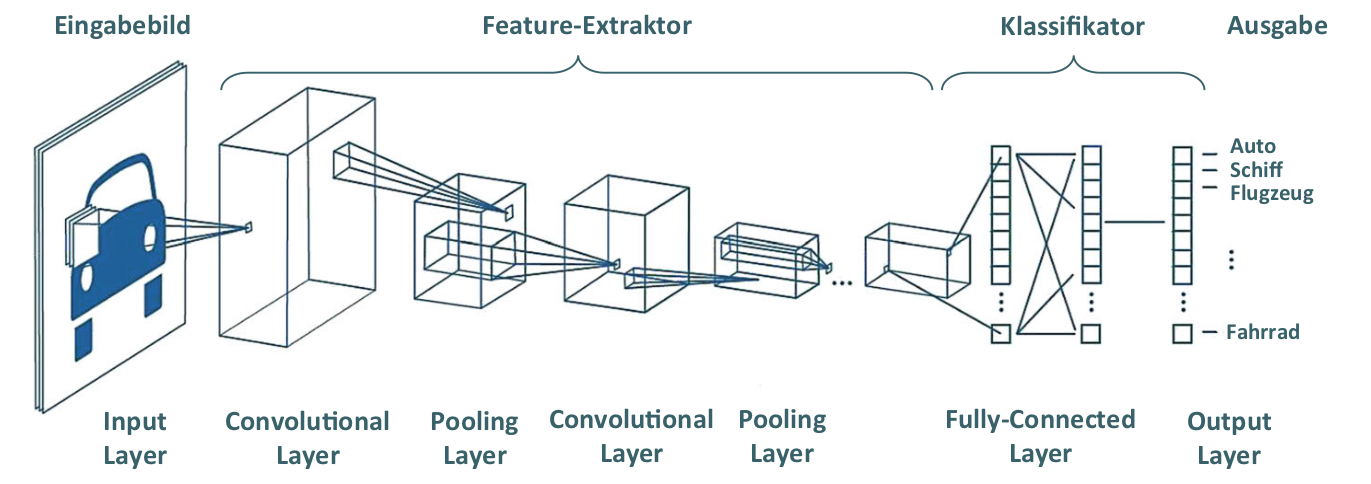
\includegraphics[width=\textwidth]{img/CNN.png}
    \caption*{Convolutional Neural Network \cite{}}
  \end{figure}
  \begin{itemize}
    \item Feature-Learning: Sequenz aus convolutional und pooling Layers
    \item Classification: Sequenz von dichten Layern
  \end{itemize}
\end{frame}

\begin{frame}
  \frametitle{Convolutional Neural Networks (CNNs)}
  \begin{figure}
    \centering
    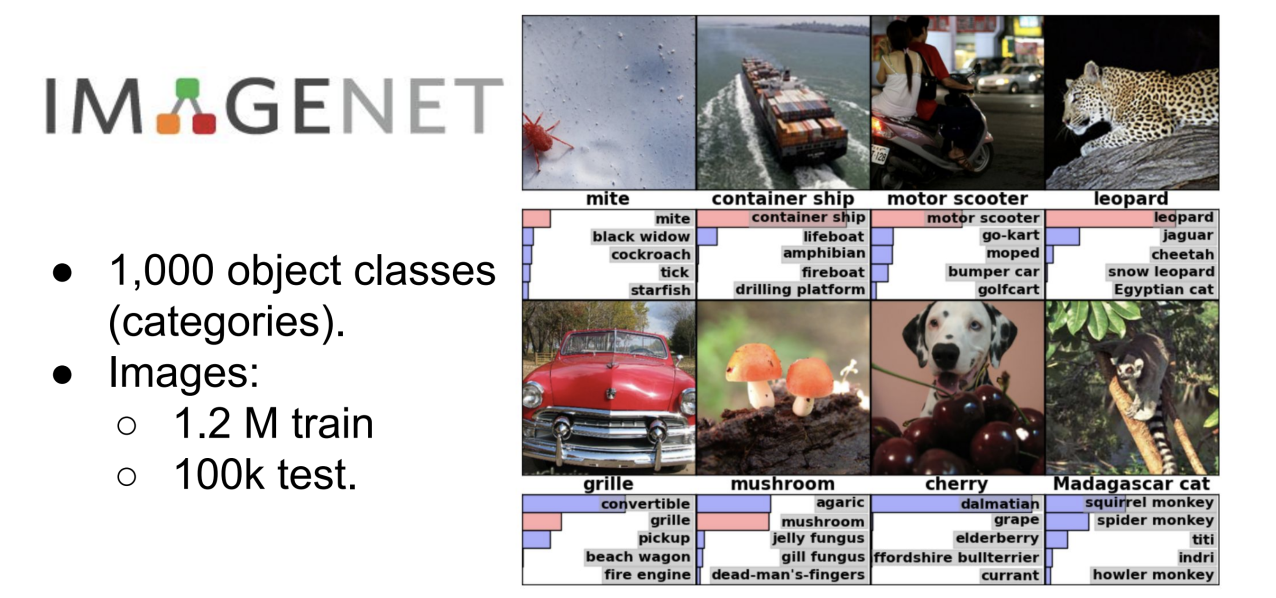
\includegraphics[width=\textwidth]{img/imagenet.png}
    \caption*{ \cite{}}
  \end{figure}
  Hier sind CNNs sehr erfolgreich!
\end{frame}

\begin{frame}
  \frametitle{Convolutional Neural Networks (CNNs)}
  \textbf{Problem}: CNNs funktionieren nur mit Euklidischen Datenstrukturen (Bilder, Text), nicht mit Graphen!
  
    \begin{figure}[H]
      \centering
      \begin{subfigure}[b]{0.49\textwidth}
        \centering
        
\includegraphics[width=\textwidth]{img/mario.png}
        \caption*{Pixelmatrix \cite{}}
      \end{subfigure}
      \begin{subfigure}[b]{0.49\textwidth}
        \centering
        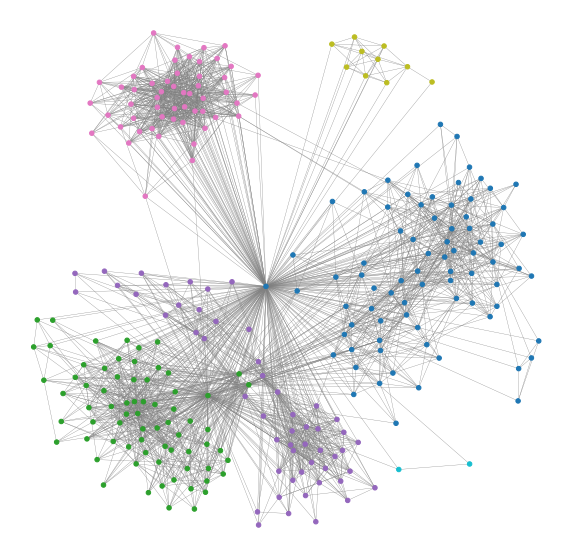
\includegraphics[width=\textwidth]{img/social_graph.png}
        \caption*{Social Graph \cite{}}
      \end{subfigure}
    \end{figure}

\end{frame}

\begin{frame}
  \frametitle{Graph Neural Networks (GNNs)}
  Ermöglichen Machine Learning auf Graphen, z.B.:
  \begin{itemize}
    \item Modellierung physikalischer Systeme
    \item Lernen molekularer Fingerabdrücke
    \item Kontrollierung von Verkehrsnetzen
    \item Freunde in sozialen Netzwerken empfehlen
  \end{itemize}
  \begin{figure}
    \centering
    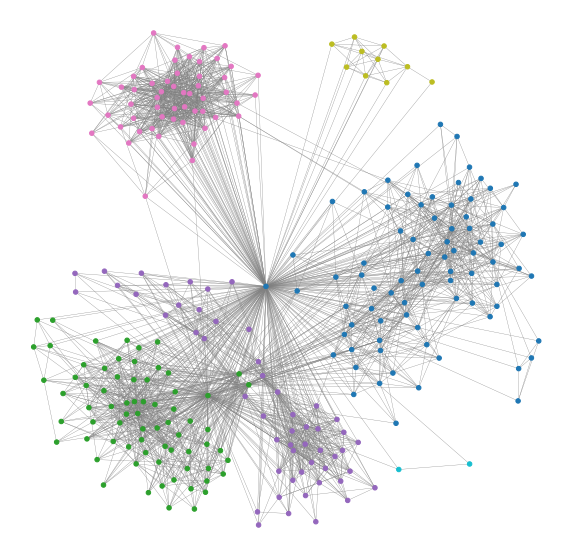
\includegraphics[width=0.4\textwidth]{img/social_graph.png}
    \caption*{Facebook Friend Network \cite{}}
  \end{figure}
\end{frame}

\begin{frame}
  \frametitle{Graph Neural Networks (GNNs)}
  Typische Aufgaben für GNNs:
  \begin{itemize}
    \item semi-supervised node classification
    \item link prediction
    \item clustering
  \end{itemize}

\end{frame}

%------------------------------------------------
\section{Robustheit}
%------------------------------------------------

\begin{frame}
  \frametitle{Robustheit von Machine Learning Modellen}

  Machine Learning Modelle sind i.A. anfällig für \textquote{Adversarial Attacks}!

  \begin{figure}
    \centering
    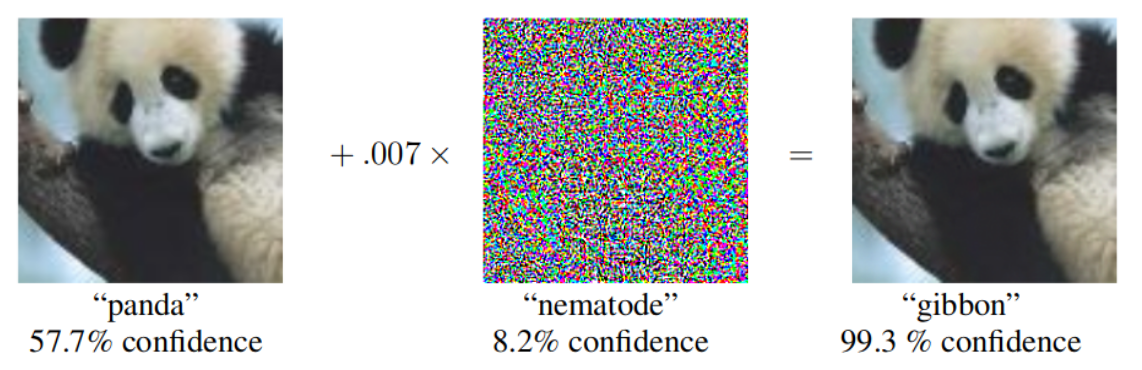
\includegraphics[width=\textwidth]{img/adversarial.png}
    \caption*{Convolutional Neural Network \cite{}}
  \end{figure}
\end{frame}

\begin{frame}
  \frametitle{Robustheit von GNNs}
  Dies gilt auch für GNNs, wobei sich zwei Arten von Angriffen unterscheiden lassen:

  \begin{itemize}
    \item Manipulation der Knoten-Attribute
    \item Manipulation der Graph-Struktur
  \end{itemize}

  \begin{figure}
    \centering
    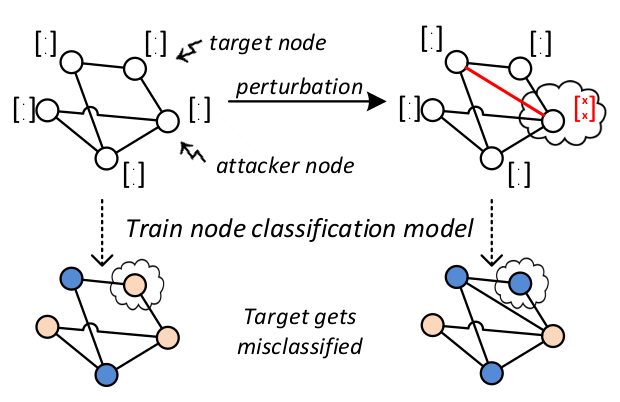
\includegraphics[width=0.7\textwidth]{img/adversarial_GNN.png}
    \caption*{ \cite{}}
  \end{figure}

\end{frame}

\begin{frame}
  \frametitle{Robustheit von GNNs}
  3 Phasen in der Literatur:
  \begin{enumerate}
    \item GNNs anfällig für \textquote{Adversarial Attacks}
    \item Verteidigungsmechanismen für bestimmte Szenarien
    \item Beweisbare Garantien für die Robustneit bestimmter Modelle
  \end{enumerate}
\end{frame}

\begin{frame}
  \frametitle{Robustheit von GNNs}
  \textbf{Zertifizierte Robustheit gegenüber Manipulationen der Knoten-Attribute:}\newline
  Wie lässt sich sicherstellen, dass kleine Änderungen am Input keine dramatischen Auswirkungen auf den Output haben?
\end{frame}

\begin{frame}
  \frametitle{Zertifizierung der Robustheit bereits trainierter GNNs}

  geg.: Graph $G = (A, X)$, Zielknoten $t$ und Parameter $\theta$\newline
  $A$: Adjazentmatrix, $X$: Knoten-Features\newline

  \textbf{Ziel}: Zertifikat für Knoten $t$ bedeutet, dass die Vorhersage für $t$ sich nach zulässigen Manipulationen nicht ändert.\newline
  $\rightarrow$ definiertes Angriffsmodell\newline

  \textquote{\textbf{Worst-Case-Margin}} $m^t$ für Knoten $t$ zwischen den Klassen $y$ und $y^{\ast}$ basierend auf einem definierten Angriffsmodell:

  \begin{gather} 
        m^t (y^*, y) := \min_{\tilde{X}} f_{\theta}^t(\tilde{X}, \dot{A})_{y^*} - f_{\theta}^t(\tilde{X}, \dot{A})_y \nonumber \\
        s.t. \quad \tilde{X} \in X_{q, Q} (\dot{X}) \nonumber
    \end{gather}
\end{frame}

\begin{frame}
  \frametitle{High-Level Idee}

  \begin{figure}[H]
    \centering
    \begin{subfigure}[b]{1\textwidth}
      \centering
      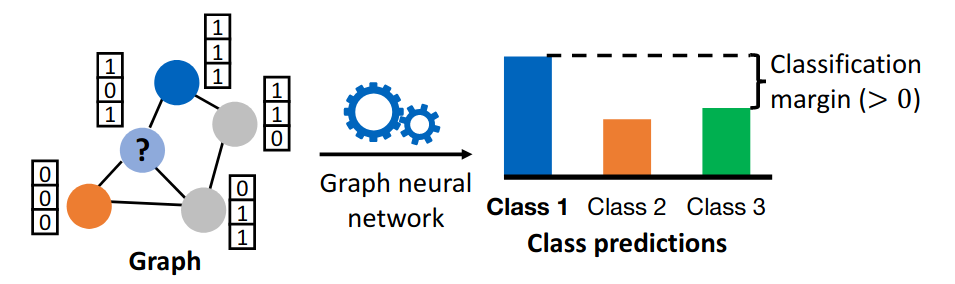
\includegraphics[width=0.75\textwidth]{img/before_pert.png}
      \caption*{\cite{}}
    \end{subfigure}
    \begin{subfigure}[b]{1\textwidth}
      \centering
      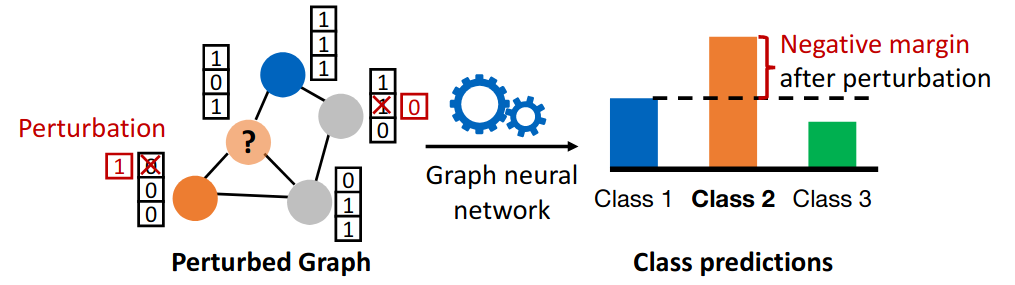
\includegraphics[width=0.75\textwidth]{img/after_pert.png}
      \caption*{\cite{}}
    \end{subfigure}
  \end{figure}
\end{frame}

\begin{frame}
  \frametitle{Lösung des Optimierungsproblems}

  \begin{itemize}
    \item Diskrete Domäne + Nicht-konvexe Aktivierungsfunktion
    \item Lösung: Mehrere Relaxationen + Berechnung unterer Schranken für das Minimum
  \end{itemize}

\end{frame}

%------------------------------------------------
\subsection{TODO}
%------------------------------------------------

%------------------------------------------------
\subsection{TODO}
%------------------------------------------------

%------------------------------------------------
\section{Fazit / Ausblick}
%------------------------------------------------

\end{document}
